\chapter{Resultate}\label{chap:r}
Die Resultate bestehen aus drei Tabellen. Jede Tabelle beschreibt die Leistung
der acht Versionen (siehe \doubleref{chap:m_var}), bezogen auf die drei definierten
Kriterien (siehe \doubleref{chap:m_eval}). Die Daten in den Tabellen
stammen aus den Tests der KI (siehe \doubleref{chap:m_auswert})
Der Unterschied in den Tabellen liegt im Datenset, mit denen die Versionen der
KI jeweils getestet sind. 
Eine Sammlung von gezeichneten Strichbildern ergänzt die Resultate. Die
Strichbilder sind dabei jeweils in Paaren angeordnet. Das linke Bild im Paar
zeigt die Vorlage aus dem Datenset und das rechte Bild zeigt die nachgezeichnete
Variante von der KI. Die Zeichnungen, die in der Sammlung
vertreten sind, sind zufällig ausgewählt aus dem Test der jeweiligen Version der
KI. Die Bilder haben einen Farbverlauf, der den zeitliche
Verlauf des Zeichnens dargestellt. Die Helligkeit eines Striches ist
proportional zu dem Step, in dem dieser gezeichnet wurde. Das bedeutet, dass
dunklere Striche früher gezeichnet werden als hellere Striche. Bewegungen des
Agents, in denen dieser nicht zeichnet, sind in den Bildern nicht erkennbar.

\newpage
\section{Tabellen}\label{chap:r_tab}
\begin{table}[!ht]
    \centering
    \caption{Testen auf MNIST Datenset | 2000 Tests}\label{tab:MNIST}
    \begin{tabular}{|l|l|l|l|}
        \hline
            ~ & Übereinstimmung \% & Erkennbarkeit \% & Geschwindigkeit \\ \hline
            Grund-Basis & 86.5 & 86.6 & 24.5 \\ \hline
            Grund-MNIST & 66.8 & 64.3 & 51.2 \\ \hline
            Grund-Speed & 86.2 & 86.6 & 25.5 \\ \hline
            Grund-MNIST-Speed & 61.4 & 55.1 & 56.8 \\ \hline
            Physik-Basis & 56.4 & 46.4 & 62.5 \\ \hline
            Physik-MNIST & 38.4 & 35.7 & 63.9 \\ \hline
            Physik-Speed & 63.0 & 58.2 & 61.2 \\ \hline
            Physik-MNIST-Speed & 29.2 & 27.3 & 63.7 \\ \hline
        \end{tabular}
\end{table}

\begin{table}[!ht]
    \centering
    \caption{Testen auf EMNIST Datenset | 2000 Tests}\label{tab:EMNIST}
    \begin{tabular}{|l|l|l|l|}
    \hline
        ~ & Übereinstimmung \% & Erkennbarkeit \% & Geschwindigkeit \\ \hline
        Grund-Basis & 86.8 & 74.5 & 38.2 \\ \hline
        Grund-MNIST & 65.2 & 45.0 & 57.4 \\ \hline
        Grund-Speed & 87.8 & 77.0 & 37.7 \\ \hline
        Grund-MNIST-Speed & 62.2 & 40.0 & 60.9 \\ \hline
        Physik-Basis & 57.6 & 32.4 & 63.5 \\ \hline
        Physik-MNIST & 43.3 & 23.6 & 63.9 \\ \hline
        Physik-Speed & 56.3 & 35.0 & 63.6 \\ \hline
        Physik-MNIST-Speed & 30.2 & 13.9 & 64.0 \\ \hline
    \end{tabular}
\end{table}

\begin{table}[!ht]
    \centering
    \caption{Testen auf QuickDraw-Datenset | 2000 Tests}\label{tab:Quickdraw}
    \begin{tabular}{|l|l|l|l|}
    \hline
        ~ & Übereinstimmung \% & Erkennbarkeit \% & Geschwindigkeit \\ \hline
        Grund-Basis & 79.1 & 80.5 & 39.1 \\ \hline
        Grund-MNIST & 57.3 & 62.5 & 59.9 \\ \hline
        Grund-Speed & 79.5 & 82.2 & 40.0 \\ \hline
        Grund-MNIST-Speed & 54.9 & 58.9 & 62.5 \\ \hline
        Physik-Basis & 48.1 & 55.7 & 63.8 \\ \hline
        Physik-MNIST & 30.5 & 38.9 & 64.0 \\ \hline
        Physik-Speed & 50.0 & 58.3 & 63.6 \\ \hline
        Physik-MNIST-Speed & 22.4 & 31.1 & 64.0 \\ \hline
    \end{tabular}
\end{table}

\newpage

\section{Bildersammlung}\label{chap:r_bild}
\begin{figure}[!ht]
    \centering
    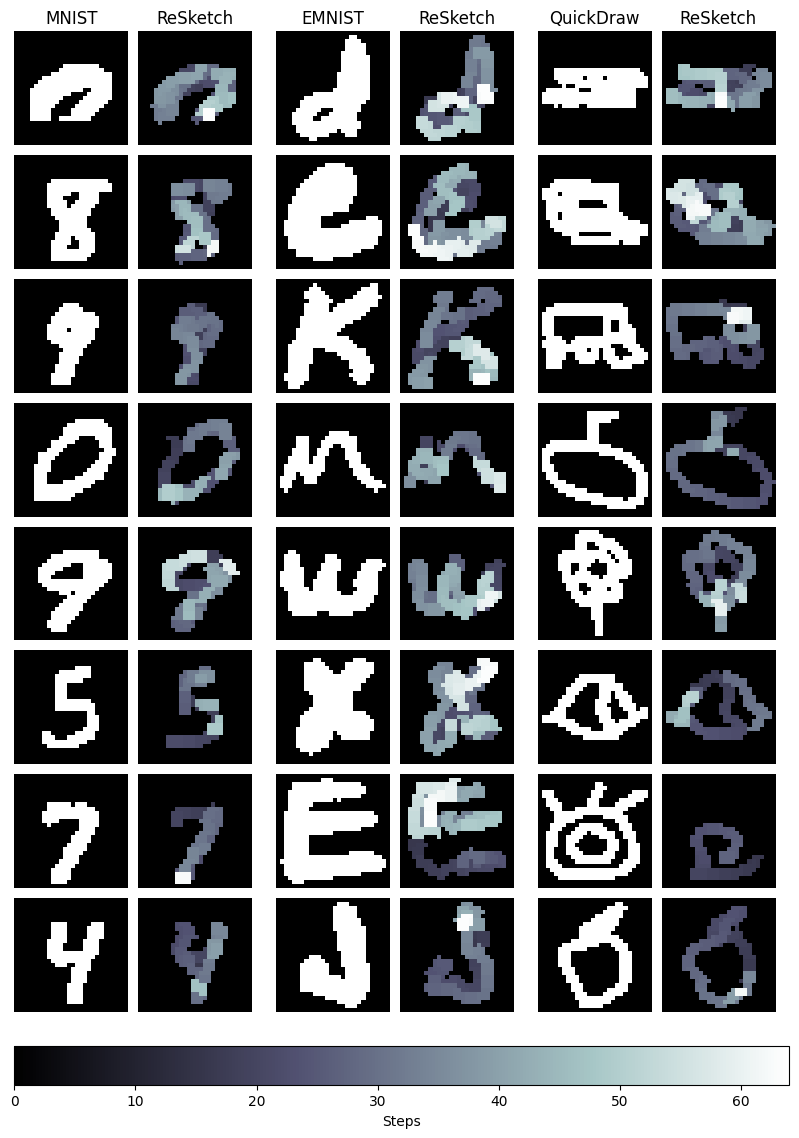
\includegraphics[width=\textwidth]{images/resultate/base-base.png}
    \caption{Grund-Basis}\label{fig:Grund-Basis}
\end{figure}

\newpage
\begin{figure}[!ht]
    \centering
    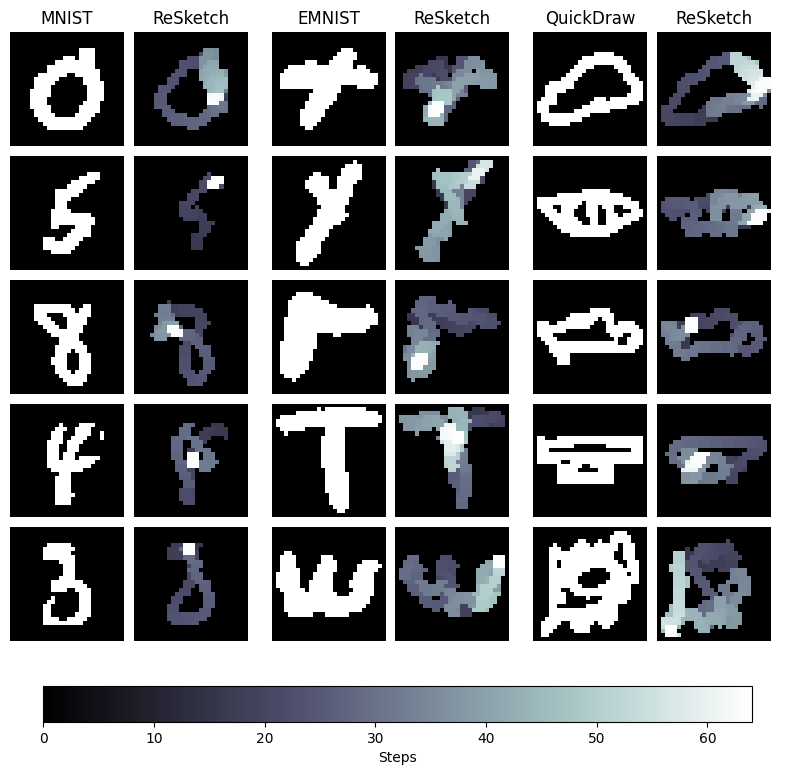
\includegraphics[width=\textwidth]{images/resultate/base-mnist.png}
    \caption{Grund-MNIST}\label{fig:Grund-MNIST}
\end{figure}

% \begin{figure}[!ht]
%     \centering
%     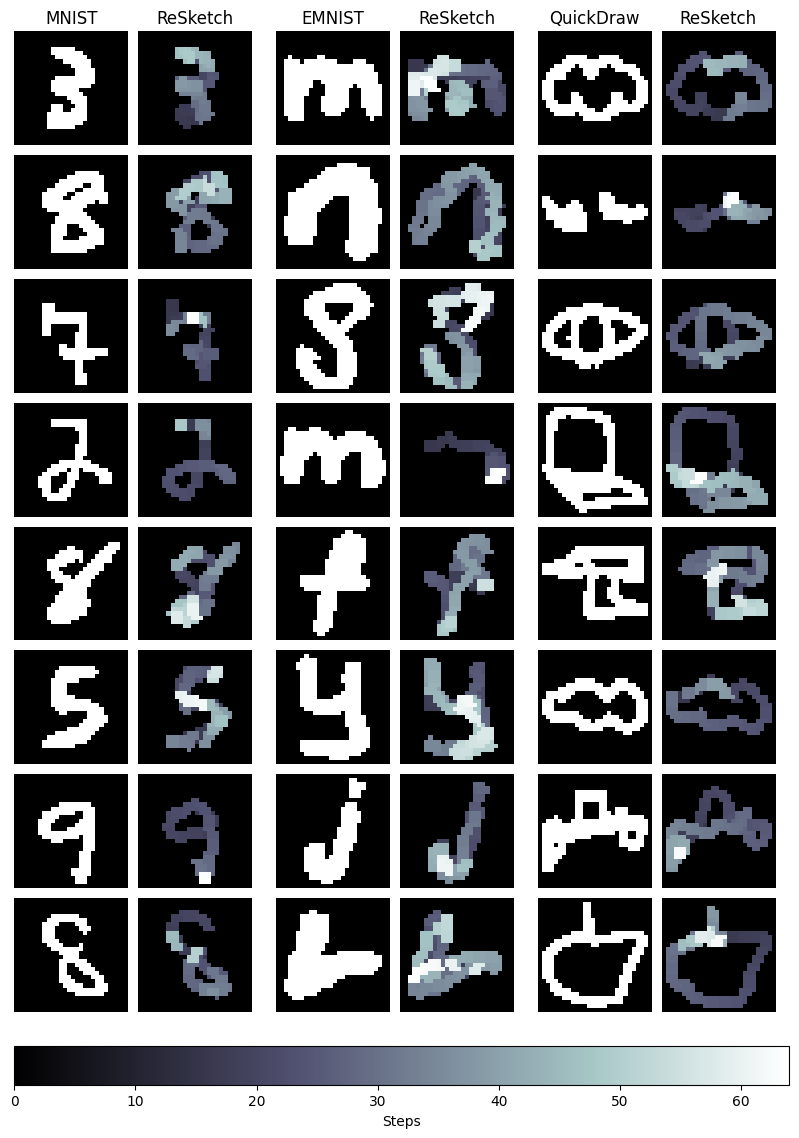
\includegraphics[width=\textwidth]{images/resultate/base-speed.png}
%     \caption{Grund-Speed}
%     \label{fig:Grund-Speed}
% \end{figure}

\begin{figure}[!ht]
    \centering
    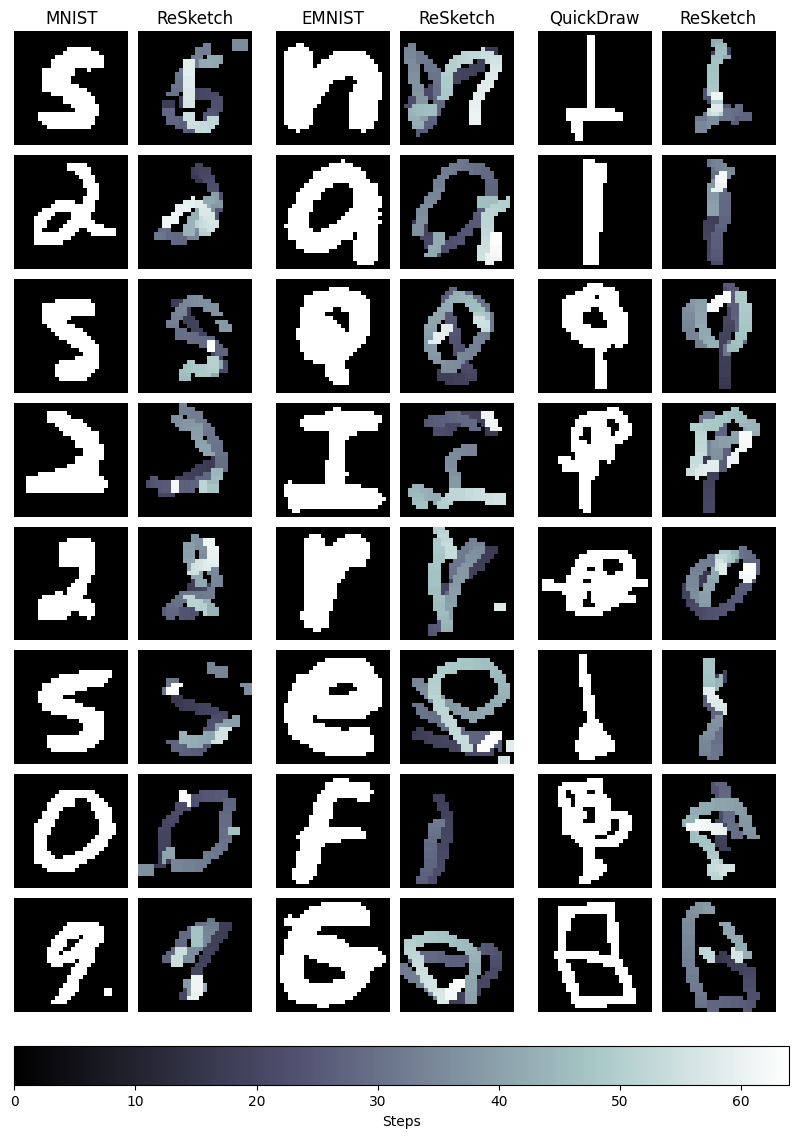
\includegraphics[width=\textwidth]{images/resultate/physics-base.png}
    \caption{Physik-Basis}\label{fig:Physik-Basis}
\end{figure}

\begin{figure}[!ht]
    \centering
    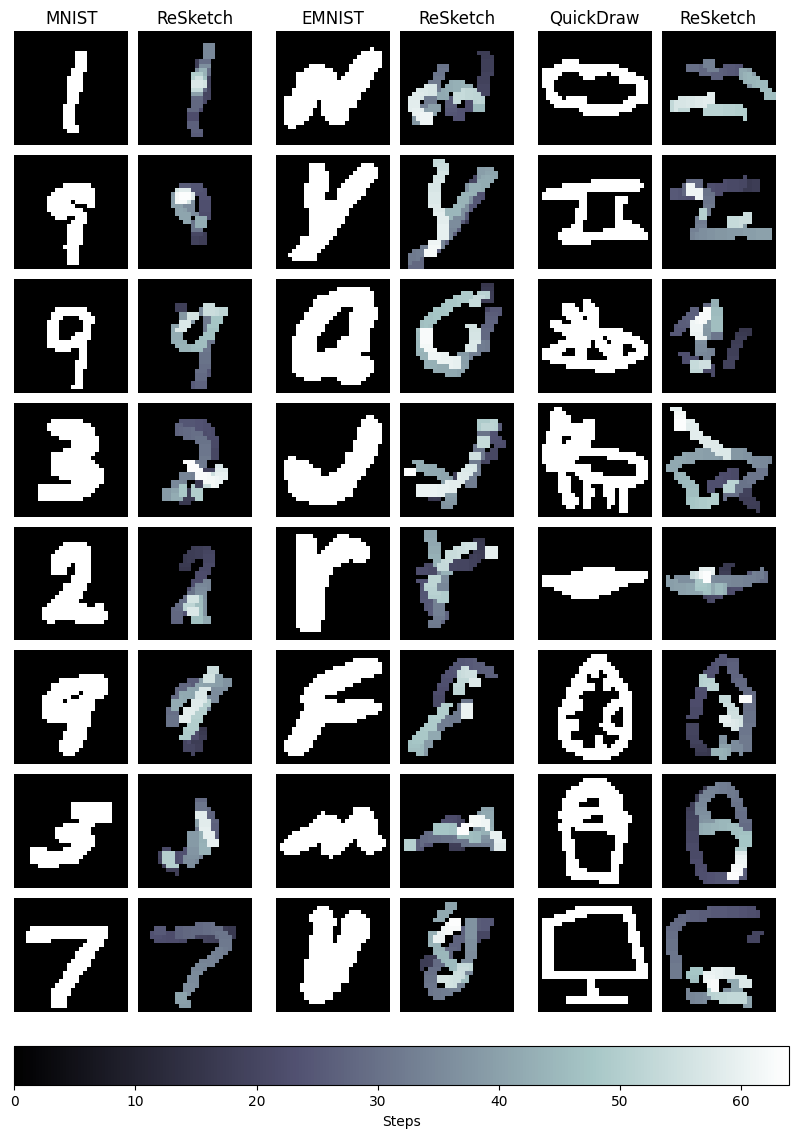
\includegraphics[width=\textwidth]{images/resultate/physics-speed.png}
    \caption{Physik-Speed}\label{fig:Physik-Speed}
\end{figure}
